\documentclass[10pt]{article}
\usepackage{icmlko}

\icmlmeta{IP 파운데이션 월드모델}{255}{수가 아니라 무엇인지}{열세 노트 만에 판이 움직였다 --- 태그의 개수가 아니라 내용으로, 그리고 새 정보로}

\begin{document}

\twocolumn[
\icmlheader

\begin{abstract}
노트 252가 프로그램 수준의 결론을 냈다 --- 축 열일곱의 여지가 $+$0.013 뿐이고
\textbf{다음 이득은 새 정보에서만 온다}. 그 말대로 했다. 노트 239가 태그
\emph{수}를 찾으며 남긴 줄 ``태그 내용 --- 수가 아니라 어떤 태그인지''가
유일하게 안 쓴 자료였다. \textbf{먼저 사후 표지를 걸러야 했다}: 학습에서
태그별 라벨 편차 아래쪽이 전부 ``완결''로 시작하는데(완결무료 $-$0.44 ·
완결일상 $-$0.25), 완결 태그가 붙은 1,271건이 \textbf{전부}
\texttt{finished=True} 다 --- 끝나야 붙는다. 각색 표지도 뺐다. 남은 태그
121종의 존재 행렬을 \textbf{학습 행으로만} 중심잡고 SVD 해서 성분을 얻고
유보는 투영만 했다 --- \textbf{라벨을 한 번도 안 본다.} 다섯 성분 중 노트
239의 채택 검사(연도 통제 상관 · 시간 다섯 조각 부호 일치)를 통과한 것은
둘이고(성분 1: $-$0.259, 5/5 · 성분 3: $-$0.184, 5/5), 기존 축과의 최대 겹침이
0.36 · 0.39 라 가드 \textbf{겹말}에서 멀다 --- 태그 수의 다시 쓰기가 아니다.
\textbf{판이 0.4569에서 0.4623으로 올랐다}(F23 $+$0.0052, $t{=}2.20$). 웹툰이
0.3805 $\to$ \textbf{0.4018}($+$0.0214, 짝 SE 0.0078, $t{=}2.75$)이고
\textbf{나머지 여덟은 넷째 자리까지 안 움직인다} --- 노트 250 · 251이 예측한
그대로다(전용 이름은 가법이다). 가드 여덟 통과. 노트 242 이후 열세 노트
만의 첫 개선이고, \textbf{모형이 아니라 자료로 얻었다.}
\end{abstract}
]

\section{남은 길이 하나였다}

노트 240--251은 판을 한 번도 못 움직였고, 노트 252가 그 이유를 쟀다 --- 축
열일곱으로 도달 가능한 천장(유보 안 CV)이 0.4697 이고 지금이 0.4569 라 여지가
$+$0.013 뿐이다. 다섯 도메인은 여지가 아예 음수다. 결론은 ``다음 이득은 새
정보에서 온다''였고, 노트 253이 ``단, 같은 자리에서 더 모으는 것은 아니다''를
붙였다.

안 쓴 자료가 딱 하나 남아 있었다. 노트 239가 웹툰 레코드에서 태그
\emph{수}를 찾아 쓰고(그리고 노트 240이 그것이 \texttt{target\_breadth} 와
같은 것임을 밝혀 취소하고) 남긴 줄이다.

\begin{quote}\small
\textbf{태그 내용} --- 수가 아니라 어떤 태그인지
\end{quote}

웹툰 2,817건에 태그 목록이 통째로 들어 있는데 개수만 쓰고 있었다.

\section{아래쪽이 전부 ``완결''이었다}

\begin{figure}[t]
\centering
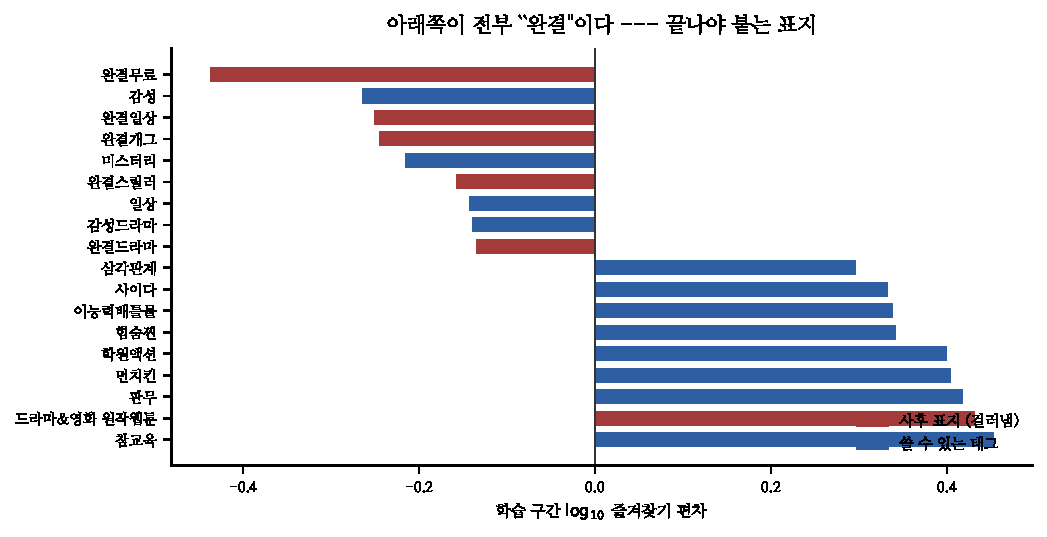
\includegraphics[width=\columnwidth]{figs/tags.pdf}
\caption{학습 구간 태그별 라벨 편차. 빨강이 걸러낸 사후 표지다.}
\end{figure}

먼저 태그별로 학습 구간 라벨 편차를 봤다. 폭이 0.89 로 신호는 뚜렷한데,
아래쪽이 수상했다 --- 완결무료 $-$0.44 · 감성 $-$0.26 · 완결일상 $-$0.25 ·
완결개그 $-$0.24.

확인했다. \textbf{``완결''이 든 태그가 붙은 1,271건은 전부
\texttt{finished=True} 다}(1,271/1,271, 100\%). 연재가 끝나야 붙는 표지이고,
노트 224가 웹툰 회차 간격을 물린 것과 같은 종류다 --- 날짜가 안 바뀌는 것과
예측 시점에 알 수 있는 것은 다른 말이다. 각색 표지(원작웹툰 · 드라마\&영화)도
같이 뺐다.

거른 뒤에도 121종이 남고 편차 폭이 0.72 다. \textbf{신호가 사후 표지에서만
온 것이 아니었다.}

\section{라벨을 한 번도 안 본다}

태그 내용을 축으로 만드는 제일 쉬운 길은 태그별 라벨 평균을 붙이는 것인데,
그것은 목표 부호화라 학습 라벨을 쓴다. 안 썼다.

태그 존재 여부 행렬(2,817 $\times$ 121)을 \textbf{학습 행으로만} 중심잡고
SVD 해서 성분을 얻고, 유보는 투영만 했다. 라벨이 한 번도 안 들어간다.

\textbf{채택 근거는 학습 구간이다}(노트 239의 규약 --- 축을 더하는 것은 자료
고침이 아니라 설계 선택이므로 유보로 정하면 안 된다).

\begin{center}\small
\begin{tabular}{lrrrl}
\hline
성분 & 연도 통제 & 조각 부호 & 설명력 & 기존 축 겹침 \\
\hline
0 & $-$0.044 & 3/5 & 8.6\% & --- \\
\textbf{1} & $\mathbf{-0.259}$ & \textbf{5/5} & 5.6\% & 0.356 \\
2 & $-$0.077 & 4/5 & 4.2\% & --- \\
\textbf{3} & $\mathbf{-0.184}$ & \textbf{5/5} & 3.8\% & 0.389 \\
4 & $-$0.111 & 5/5 & 3.4\% & --- \\
\hline
\end{tabular}
\end{center}

둘이 통과했다(성분 4는 연도 통제 상관이 문턱 아래). 겹침이 0.36 · 0.39 로
가드 \textbf{겹말}(노트 240)의 0.95 에서 멀다 --- \textbf{태그 수의 다시
쓰기가 아니다.} 노트 240에서 데인 자리를 이번엔 먼저 확인했다.

\textbf{이름은 웹툰 전용으로 준다}(노트 250 · 251). 웹툰만 갖는 축을 공유
이름으로 주면 결국 전용 열이 되면서 ``일부에게만 준 공유 열''이라는 존재하지
않는 중간을 만든다.

\section{판이 움직였다}

\begin{figure}[t]
\centering

\includegraphics[width=\columnwidth]{figs/board.pdf}
\caption{도메인별. 웹툰만 오르고 나머지는 안 흔들린다.}
\end{figure}

\begin{center}\small
\begin{tabular}{lrr}
\hline
 & 17축 & 19축 \\
\hline
F21 능형 & 0.4381 & 0.4361 \\
F18 나무 & 0.4480 & 0.4532 \\
\textbf{F23 판} & \textbf{0.4569} & \textbf{0.4623} \\
\hline
\end{tabular}
\quad
\begin{tabular}{lr}
\hline
짝 차 & $t$ \\
\hline
$-$0.0020 & $-$1.06 \\
$+$0.0053 & $+$1.42 \\
$\mathbf{+0.0052}$ & $\mathbf{+2.20}$ \\
\hline
\end{tabular}
\end{center}

도메인별로 보면 더 깨끗하다.

\begin{center}\small
\begin{tabular}{lrrr}
\hline
도메인 & 17축 & 19축 & 차 \\
\hline
\textbf{웹툰} & 0.3805 & \textbf{0.4018} & $\mathbf{+0.0214}$ \\
애니 & 0.4873 & 0.4873 & $+$0.0000 \\
모바일 & 0.5374 & 0.5379 & $+$0.0005 \\
세계애니 & 0.5199 & 0.5199 & $+$0.0000 \\
게임 & 0.6397 & 0.6397 & $+$0.0000 \\
\hline
\end{tabular}
\end{center}

웹툰의 짝 SE 가 0.0078 이라 $t{=}2.75$ 다. \texttt{rank.spread}(노트 247 ·
248)로 보면 \textbf{진짜 총량 0.0058 에 순 $+$0.0053} --- 상쇄가 없다.
\textbf{나머지 여덟이 안 흔들리는 것은 노트 250 · 251이 예측한 그대로다} ---
전용 이름 열은 가법이라(교차항/부분합 0.18) 남에게 안 샌다. 노트 246의
``남이 치른다''가 여기서는 안 일어난다.

가드 여덟이 다 통과한다. \textbf{시점}이 특히 중요했는데, 태그는 지금 긁은
스냅샷이라 위키 · 검색처럼 창을 못 자른다. 사전으로 보는 근거는 노트 239가
이미 재 뒀다 --- 쌓이는 것이라면 옛 작품이 태그가 더 많아야 하는데 태그 수가
연도와 $+$0.369 다(신작이 더 많다). 누적이 아니라 태깅 체계의 시대 효과이고,
쌓이는 유일한 표지인 ``완결''은 위에서 뺐다.

\section{열세 노트 만이다}

판 이동을 적어 둔다: 노트 242의 0.4569 이후 노트 243--254 열두 편이 판을
한 자리도 못 움직였고, 이번이 \textbf{0.4623} 이다.

그 열두 편이 헛되지 않았다는 것이 이 노트의 두 번째 이야기다. 이번 축을
놓을 때 쓴 것이 전부 거기서 나왔다 --- 겹말 확인(240) · 전용 이름 선택
(250 · 251) · 상쇄 점검(247 · 248) · 학습 구간 채택 규약(239) · 그리고
무엇보다 \textbf{어디를 파야 하는지}(252). 판이 안 움직인 열두 편이 판을
움직인 한 편의 도구가 됐다.

\paragraph{남은 것}
\begin{center}\small
\begin{tabular}{ll}
\hline
갈래 & 왜 \\
\hline
세계애니 · 만화 태그 & 같은 필드가 있다. 두 도메인 몫이 12\% \\
성분 0 · 2 & 부호 3/5 · 4/5 로 떨어졌다. 조각을 바꾸면? \\
태그 내용 $\times$ 다른 도메인 & 게임 · 모바일에 장르 문자열이 있나 \\
웹툰 남은 여지 & CV 천장 0.431 이었는데 0.402 까지 왔다 \\
\hline
\end{tabular}
\end{center}

\paragraph{규약} 노트 252의 ``새 정보에서만 온다''에 한 줄 붙인다 ---
\textbf{안 쓴 자료를 찾을 때는 이미 쓰는 필드의 \emph{다른 면}을 먼저 본다.}
태그는 2년 동안 판에 있었지만 개수로만 있었다. 새로 긁을 것이 없어도
새 정보가 남아 있을 수 있다.

\end{document}
